% @Author: AnthonyKenny98
% @Date:   2020-03-01 19:39:42
% @Last Modified by:   AnthonyKenny98
% @Last Modified time: 2020-04-10 17:17:19

% Intro
Recall the computer implementation hierarchy in Figure \ref{fig:computerHierarchy}, made up of user-level applications, programming languages, the instruction set architecture, and the processor. Computer Architecture encompasses the two lower levels of this hierarchy. It comprises the design of the Instruction Set Architecture and Microarchitecture of a computer. Earlier, the Instruction Set was described as the ``translator'' between software and the processor. The \textbf{Instruction Set} is in reality a document defining the behaviour of a computer. The \textbf{Microarchitecture} is the implementation the \gls{ISA}; the physical computer processor that behaves in the way defined by the \gls{ISA}.

% @Author: AnthonyKenny98
% @Date:   2020-04-09 10:47:05
% @Last Modified by:   AnthonyKenny98
% @Last Modified time: 2020-04-09 11:21:26
\begin{figure}[H]
\begin{centering}
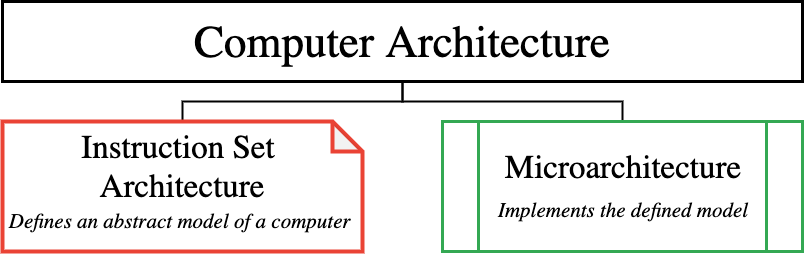
\includegraphics[width=0.7\linewidth]{chapters/chapter4/img/architecture.png}
\mycaption{Overview of the Field of Computer Architecture}{}
\end{centering}
\end{figure}

\subsection{Instruction Set Architecture}
    An \glsfirst{ISA} is an abstract model of a computer. On a broad level, it defines the instructions that it can execute, along with the data types, memory model, and registers of the computer. \\
    In more human terms, it can be thought of as a ``contract'' between hardware and software developers. It is a list of all the instructions that a computer will implement; all software will be compiled into these instructions, and all processors will be built to implement these instructions.

    % @Author: AnthonyKenny98
% @Date:   2020-04-09 10:47:05
% @Last Modified by:   AnthonyKenny98
% @Last Modified time: 2020-04-11 01:21:24
\begin{figure}[H]
\begin{centering}
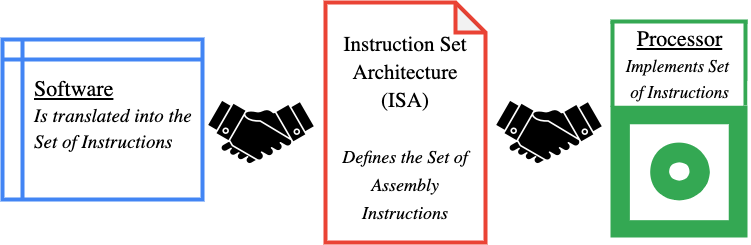
\includegraphics[width=\linewidth]{chapters/chapter4/img/contract.png}
\mycaption{The ISA is a Contract Between Software and Hardware Developers}{}
\end{centering}
\end{figure}

    The two most important things that an \gls{ISA} defines are a computer's \textbf{instructions} and \textbf{registers}.
    Instructions are the operations the computer can execute. Registers can be thought of as slots in which the processor can store values, such as in Figure \ref{fig:regfile}. 

    % @Author: AnthonyKenny98
% @Date:   2020-04-10 16:04:25
% @Last Modified by:   AnthonyKenny98
% @Last Modified time: 2020-04-10 17:16:59
\begin{figure}[H]
\begin{center}
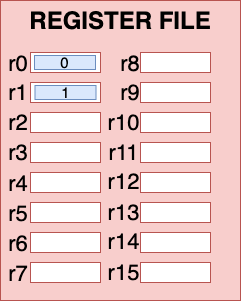
\includegraphics[width=0.5\linewidth]{chapters/chapter4/img/regfile.png}
\mycaption{Abstract Concept of a Register File}{ as a collection of slots in which a processor can store values.}
\label{fig:regfile}
\end{center}
\end{figure}

    \noindent Consider the RISC-V assembly instruction, \texttt{add}: 
    \begin{verbatim}
    add rd, rs1, rs2
    \end{verbatim}

    \noindent\texttt{rs1} and \texttt{rs2} stand for Source Register 1 and Source Register 2. \texttt{rd} stands for Destination Register. This instruction computes \texttt{rs1} $+$ \texttt{rs2} and stores the result in \texttt{rd}. For example, consider an assembly program with the following three instructions and the register file from Figure \ref{regfile} (note that r0 is initialized to the value of 0 and r1 to the value of 1.)

    \begin{verbatim}
    add r2, r1, r1
    add r3, r1, r2
    add r4, r2, r2
    \end{verbatim}
    The first instruction computes \texttt{r1} + \texttt{r1} and stores the result in \texttt{r2}. Since \texttt{r1} is initialized to 1, this results in the value of 2 being stored in \texttt{r2}. The second instruction stores \texttt{r1} + \texttt{r2} in \texttt{r3}. Finally, the last instruction stores \texttt{r2} + \texttt{r2} in \texttt{r4}. When the program finishes executing, registers 2, 3, and 4 have all been updated, as shown in Figure \ref{fig:regfileupdated}. I.e. new values have been stored in the computers slots.

    % @Author: AnthonyKenny98
% @Date:   2020-04-10 16:04:25
% @Last Modified by:   AnthonyKenny98
% @Last Modified time: 2020-04-10 17:17:05
\begin{figure}[H]
\begin{center}
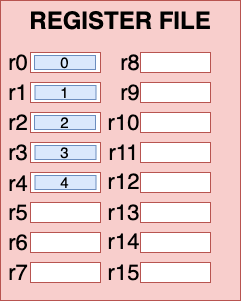
\includegraphics[width=0.5\linewidth]{chapters/chapter4/img/regfileupdated.png}
\mycaption{Updated Abstract Register File}{ after having registers 2, 3, and 4 updated by an assembly program.}
\label{fig:regfileupdated}
\end{center}
\end{figure}

    To recap, the above is an explanation of instructions and registers. The Instruction Set Architecture defines what registers a processor has and what instructions it can execute.

\subsection{Microarchitecture}

    % @Author: AnthonyKenny98
% @Date:   2020-03-01 20:09:46
% @Last Modified by:   AnthonyKenny98
% @Last Modified time: 2020-04-03 13:32:58
\begin{figure}[H]
    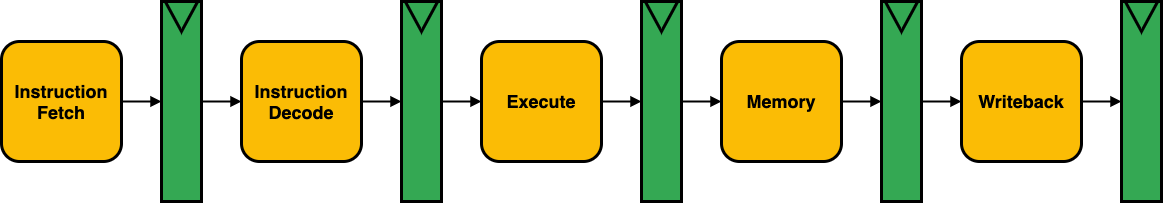
\includegraphics[draft=false,width=\linewidth]{chapters/chapter4/img/RISC-Datapath.png}
    \caption{5-Stage \gls{RISC} Datapath}
    \label{fig:RISC-Datapath}
\end{figure}

    Microarchitecture refers to the actual implementation of the behaviour defined in the \gls{ISA}. It is the design of the actual computer processor. Processors are typically implemented in stages, where each instruction goes through a certain number of stages to complete execution.
    Figure \ref{fig:RISC-Datapath} shows the most simple layout of a 5-stage \gls{RISC} Datapath (\gls{RISC} is the computing principle on which RISC-V was founded. Appendix \ref{section:philv_appendix_RISC} gives a background on RISC). In the \textbf{Instruction Fetch} stage, the processor gets the next instruction from memory for it to be decoded in the \textbf{Instruction Decode} stage. Here, the instruction is split into its constituent parts and has certain minor operations performed that are neccesary for the next stage. The \textbf{Execution} stage is where most computation occurs. This is where the \glsfirst{ALU} resides, and the result of this computation goes to the \textbf{Memory} stage. This is where values are stored into or loaded from the processor's memory, these values, or the values from the Execution stage, are saved to one of the processor's registers in the \textbf{Writeback} stage. 
